\documentclass[11pt,a4paper]{article}
\usepackage[T1]{fontenc}
\usepackage[margin=22mm]{geometry}
\usepackage{graphicx,booktabs,amsmath}
\setlength{\parindent}{0pt}\setlength{\parskip}{5pt}
\begin{document}
\section*{NAUSICA ion-frame noise with the revised transistor model}
The calculation uses the supplied Spice2 transistor card with NOIMOD=2.
The derived copy corrects NMOS NOIBE to NOIB and closes both model parameter
lists. Device dimensions, biases and numerical model parameters are unchanged.
The coefficients are treated as inputs provided by Rogelio, without independent
process calibration.

The external pad capacitance is 1.25 pF, with intrinsic MOS capacitances
added by SPICE. The feedback capacitance is 3 fF and the temperature is
293.15 K. Uniform mean ion arrivals extend over 10 ms. The input is
the saved current for a 0.5 mm square pad in a grounded plane, integrated along
a finite 5 mm approach without charge renormalization.

Centered voltage averages of 300 $\mu$s are taken at the frame boundaries.
The corrected voltage difference is $D=-(\overline V_n-\alpha\overline V_{n-1})$,
with $\alpha=\exp(-\Delta t/\tau_0)$ and $\tau_0=0.3$ s.
The circuit's actual discharge is determined by the feedback transistor.
The one-sided stationary output noise is integrated from 0.1 Hz to 1 MHz
with the same averaging and subtraction filter. ADC noise is excluded.

The signal calibration is 15.469 $\mu$V per ion, unchanged from the previous
model. The filtered noise is 4.577 mV RMS, giving
\[
 \mathrm{ENC}=295.86\ e\ \mathrm{RMS}.
\]
The previous model gave 40.47 electrons RMS. Flicker contributes
289.94 electrons RMS and thermal sources contribute 58.84 electrons RMS,
combined in quadrature. Flicker accounts for 96.04\% of the filtered
noise variance. M4 contributes 81.77\% of the total variance.

Direct LTspice transients give $S/N=4.99985$ for 1484 ions and
$S/N=5.003208$ for 1485 ions. Thus the verified integer threshold is
1485 ions for $S/N>5$. The linear calibration predicts 1480 ions;
the direct test includes the small finite-amplitude change of response.

\begin{center}
\begin{tabular}{rrrr}\toprule
Average ($\mu$s) & Gain ($\mu$V/ion) & Noise (mV RMS) & ENC ($e$ RMS)\\\midrule
180 & 15.498 & 4.848 & 312.84 \\
200 & 15.494 & 4.793 & 309.32 \\
250 & 15.482 & 4.674 & 301.89 \\
300 & 15.469 & 4.577 & 295.86 \\
350 & 15.455 & 4.494 & 290.77 \\
\bottomrule\end{tabular}
\end{center}
\begin{center}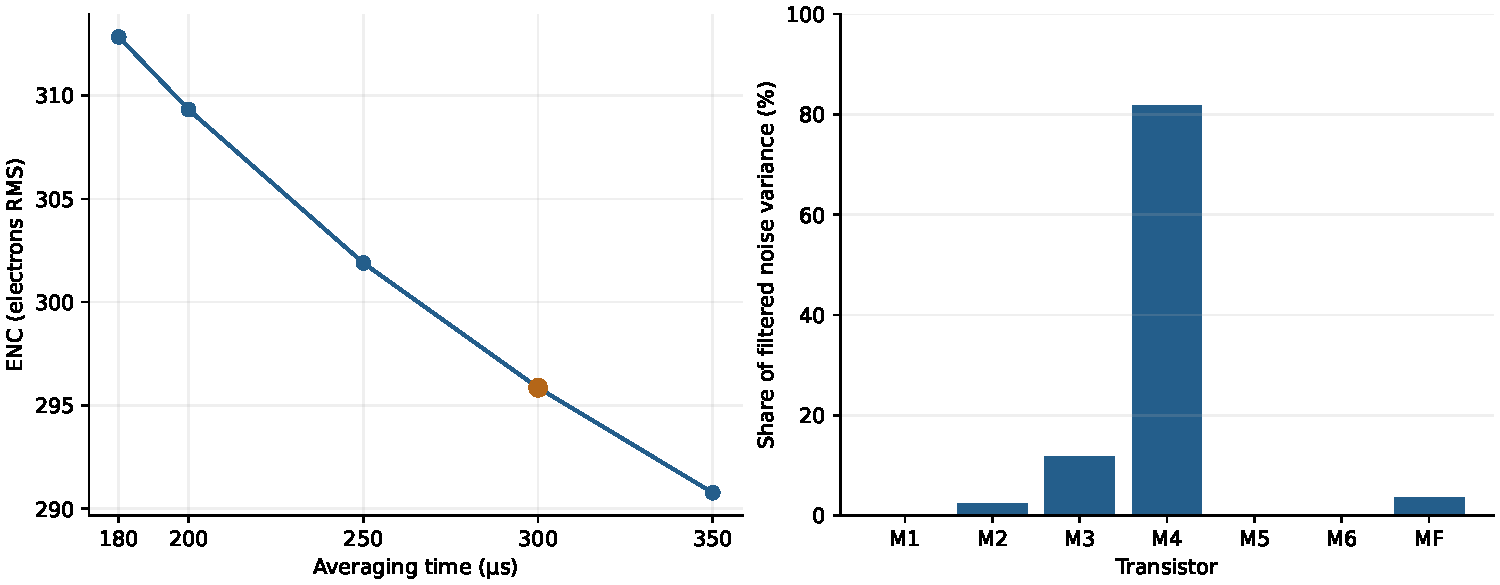
\includegraphics[width=\linewidth]{enc_and_sources.pdf}\end{center}

\subsection*{Validation}
Independent finite-path charge, halved transient steps, doubled spectral density
and quadrature orders 8 and 16 are checked. Relative errors are respectively
1.22e-15, 2.99e-07, 1.54e-07 and 6.11e-14. The two adjacent integer
counts remain on opposite sides of $S/N=5$ at both transient resolutions;
the combined numerical refinement estimate is less than one tenth of their
distance from the boundary. The total noise variance agrees with the sum of
the transistor variances. Separately integrated flicker and thermal variances
close to the integrated total within 1.05e-07 relative error.

The reproducible pipeline is \texttt{make spice2-enc}; HDF5 results, input hashes,
source waveforms, derived decks and solver logs are saved in the repository.
\end{document}
